\chapter{Units Overview, Commands and Events Description}

This chapter describes all functional blocks (units) implemented in GEX, version 1.0. The term ``unit'' will be used here to refer to both unit types (drivers) or their instances where the distinction is not important.

Each unit's description will be accompanied by a corresponding snippet from the configuration file, and a list of supported commands and events. The commands and events described here form the payload of TinyFrame messages 0x10 (Unit Request) and 0x11 (Unit Report), as described in section \ref{sec:unit_requests_reports}. The number in the first column of the command (or event) tables, marked as ``Code'', is the command number (or report type) used in the payload to identify how the message data should be treated.

When the request or response payload is empty, it's omitted from the table. The same applies to commands with no response, in which case adding 0x80 to the command number triggers a SUCCESS response after the command is finished.

\section{Naming Conventions and Common Principles}

\subsection{Unit Naming}

Unit types are named in uppercase (e.g. SPI, 1WIRE, NPX) in the INI file and in the list of units. Unit instances can be named in any way the user desires; using lowercase makes it easier to distinguish them from unit types. It is advisable to use descriptive names, e.g. not ``pin1'' but rather ``button''.

\subsection{Packed Pin Access}

Several units facilitate an access to a group of GPIO pins, such as the digital input and output units, or the SPI unit's slave select pins. The STM32 microcontroller's ports have 16 pins each, most of which can be configured to one of several alternate functions (e.g. SPI, PWM outputs, ADC input). As a consequence, it's common to be left with a discontiguous group of pins after assigning all the alternate functions needed by an application.

\begin{figure}[h]
	\centering
	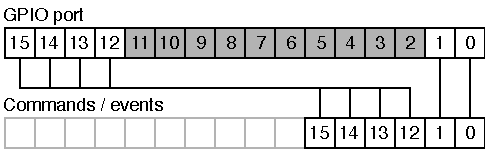
\includegraphics[scale=1] {img/pin-packing.pdf}
	\caption{\label{fig:pin-packing}Pin packing}
\end{figure}

For instance, we could only have the pins 0, 1, 12--15 available on a \gls{GPIO} port. GEX provides a helpful abstraction to bridge the gaps in the port: The selected pins are packed together and represented, in commands and events, as a block of six pins (0x3F) instead of their original positions in the register (0xF003). This scheme is shown in figure \ref{fig:pin-packing}. The translation is done in the unit driver and works transparently, as if the block of pins had no gaps---all the referenced pins are updated simultaneously without glitches. Where pin numbers are used, the order in the packed word should be provided---in our example, that would be 0--5, counting from the least significant bit.


% here are the unit sections, all following a common pattern
\section{Digital Output}

The digital output unit provides a write access to one or more pins of a \gls{GPIO} port. This unit additionally supports pulse generation on any of its pins; this is implemented in software, with timing derived from the system timebase, in order to support pulses on all pins regardless of hardware \gls{PWM} support. Pins in commands are expressed in the packed format (\cref{sec:packedpins}).

\subsection{Digital Output Configuration}

\begin{inicode}
[DO:out@1]
# Port name
port=A
# Pins (comma separated, supports ranges)
pins=0
# Initially high pins
initial=
# Open-drain pins
open-drain=
\end{inicode}

\subsection{Digital Output Commands}

\begin{cmdlist}

	0 & \cname{WRITE} Write to all pins
	& \begin{cmdreq}
		\cfield{u16} new value
	\end{cmdreq} \\

	1 & \cname{SET} Set selected pins to 1
	& \begin{cmdreq}
		\cfield{u16} pins to set
	\end{cmdreq} \\

	2 & \cname{CLEAR} Set selected pins to 0
	& \begin{cmdreq}
		\cfield{u16} pins to clear
	\end{cmdreq} \\

	3 & \cname{TOGGLE} Toggle selected pins
	& \begin{cmdreq}
		\cfield{u16} pins to toggle
	\end{cmdreq} \\

	4 & \cname{PULSE}
	Generate a pulse on the selected pins. The microsecond scale may be used only for 0--999\,$\mu$s.
	& \begin{cmdreq}
		\cfield{u16} pins to pulse
		\cfield{u8} active level (0, 1)
		\cfield{u8} scale: 0-ms, 1-$\mu$s
		\cfield{u16} duration
	\end{cmdreq}

\end{cmdlist}

\section{Digital Input}

The digital input unit is the input counterpart of the digital output unit. In addition to reading the immediate digital levels of the selected pins, this unit can report asynchronous events on a pin change. 

All pins of the unit may be configured either for a rising, falling, or any change detection; due to a hardware limitation, the same pin number may not be used for event detection on different ports (e.g. A1 and B1) at the same time. In order to receive a pin change event, we must arm the pin first, using a command; it can be armed for a single event, or it may be re-armed automatically with a hold-off time. It is, further, possible to automatically arm selected pins on start-up, removing the need to arm them e.g. after the module restarts or is re-connected.

\subsection{Digital Input Configuration}

\begin{inicode}
[DI:in@2]
# Port name
port=A
# Pins (comma separated, supports ranges)
pins=10-8,3-0
# Pins with pull-up
pull-up=10,9
# Pins with pull-down
pull-down=0

# Trigger pins activated by rising/falling edge
trig-rise=10
trig-fall=
# Trigger pins auto-armed by default
auto-trigger=10
# Triggers hold-off time (ms)
hold-off=100
\end{inicode}

\subsection{Digital Input Events}

\begin{cmdlist}

	0 & \cname{PIN\_CHANGE}
	A pin change event. The payload includes a snapshot of all configured pins captured immediately after the change was registered.
	& \begin{cmdpld}
		\cfield{u16} changed pins
		\cfield{u16} port snapshot
	\end{cmdpld}

\end{cmdlist}

\subsection{Digital Input Commands}

\begin{cmdlist}
	0 & \cname{READ} Read the pins
	& \begin{cmdresp}
		\cfield{u16} pin states
	\end{cmdresp} \\

	1 & \cname{ARM\_SINGLE} Arm for a single event
	& \begin{cmdreq}
		\cfield{u16} pins to arm
	\end{cmdreq} \\

	2 & \cname{ARM\_AUTO} Arm with automatic re-arming after each event
	& \begin{cmdreq}
		\cfield{u16} pins to arm
	\end{cmdreq} \\

	3 & \cname{DISARM} Dis-arm selected pins
	& \begin{cmdreq}
		\cfield{u16} pins to dis-arm
	\end{cmdreq}
\end{cmdlist}

\section{SIPO (Shift Register) Unit}

The shift registers driver unit is designed for the loading of data into \textit{serial-in, parallel-out} (SIPO) shift registers, such as 74HC4094 or 74HC595. Those are commonly used to control segmented LED displays, LED matrices etc.

This unit handles both the \textit{Shift} and \textit{Store} signals and is capable of loading multiple shift registers simultaneously, reducing visible glitches in the display. It's also possible to set the data lines to arbitrary level(s) before sending the Store pulse, which can be latched and used for some additional feature of the LED display, such as brightness control.


\subsection{SIPO Configuration}

\begin{inicode}
[SIPO:display@9]
# Shift pin & its active edge (1-rising,0-falling)
shift-pin=A1
shift-pol=1
# Store pin & its active edge
store-pin=A0
store-pol=1
# Clear pin & its active level
clear-pin=A2
clear-pol=0
# Data port and pins
data-port=A
data-pins=3
\end{inicode}

\subsection{SIPO Commands}

\begin{cmdlist}
	0 & \cname{WRITE}
	Load the shift registers and leave the data outputs in the ``trailing data'' state before sending the Store pulse.
	&
	\begin{cmdreq}
		\cfield{u16} trailing data
		\item For each output (same size)
		\begin{pldlist}
			\cfield{u8[]} data to load
		\end{pldlist}
	\end{cmdreq}
	\\

	1 & \cname{DIRECT\_DATA}
	Directly write to the data pins (same like the DO unit's WRITE command)
	&
    \begin{cmdreq}
		\cfield{u16} values to write
	\end{cmdreq} \\

	2 &
	\cname{DIRECT\_CLEAR}
	Pulse the Clear pin, erasing the registers' data & \\

	3 &
	\cname{DIRECT\_SHIFT}
	Pulse the Shift pin & \\

	4 &
	\cname{DIRECT\_STORE}
	Pulse the Store pin & \\
\end{cmdlist}




\section{NeoPixel Unit}

The NeoPixel unit implements the protocol needed to control a digital \gls{LED} strip with WS2812, WS2811, or compatible \gls{LED} driver chips. The protocol timing is implemented in software, therefore it is available on any GPIO pin of the module.

The color data can be loaded in five different format: as packed bytes, or as the little-endian or big-endian encoding of colors in the 32-bit format 0x00RRGGBB or 0x00BBGGRR. This data format is convenient when the colors are already represented by an array of 32-bit integers.

\subsection{NeoPixel Configuration}

\begin{inicode}
[NPX:neo@3]
# Data pin
pin=A0
# Number of pixels
pixels=32
\end{inicode}

\subsection{NeoPixel Commands}

\begin{cmdlist}
	0 & \cname{CLEAR}
	Switch all \glspl{LED} off (sets them to black) & \\

	1 & \cname{LOAD}
	Load a sequence of R,G,B bytes
	& \begin{cmdreq}
		\item For each LED:
		\begin{pldlist}
			\cfield{u8} red
			\cfield{u8} green
			\cfield{u8} blue
		\end{pldlist}
	\end{cmdreq} \\

	4 & \cname{LOAD\_U32\_ZRGB}
	Load 32-bit big-endian 0xRRGGBB (0,R,G,B)
	& \begin{cmdreq}
		\cfield{u32[]} color data BE
	\end{cmdreq} \\

	5 & \cname{LOAD\_U32\_ZBGR}
	Load 32-bit big-endian 0xBBGGRR (0,B,G,R)
	& \begin{cmdreq}
		\cfield{u32[]} color data BE
	\end{cmdreq} \\

	6 & \cname{LOAD\_U32\_RGBZ}
	Load 32-bit little-endian 0xBBGGRR (R,G,B,0)
	& \begin{cmdreq}
		\cfield{u32[]} color data LE
	\end{cmdreq} \\

	7 & \cname{LOAD\_U32\_BGRZ}
	Load 32-bit little-endian 0xRRGGBB (B,G,R,0)
	& \begin{cmdreq}
		\cfield{u32[]} color data LE
	\end{cmdreq} \\

	10 & \cname{GET\_LEN}
	Get number of \glspl{LED} in the strip
	& \begin{cmdresp}
		\cfield{u16} number of \glspl{LED}
	\end{cmdresp} \\

\end{cmdlist}




\section{SPI Unit}

The SPI unit provides access to one of the microcontroller's SPI peripherals. It can be configured to use any of the different speeds, clock polarity and phase settings available in its control registers. The unit handles up to 16 slave select (NSS) signals.

Both write-only and read-write (query) transactions are implemented.

\todo[inline]{Query diagram}

\section{\IIC Unit}

The \gls{I2C} unit provides access to one of the microcontroller's \gls{I2C} peripherals. More on the \IIC bus can be found in \cref{sec:theory-i2c}.

The unit can be configured to use either of the three standard speeds (Standard, Fast and Fast+) and supports both 10-bit and 7-bit addressing. 10-bit addresses can be used in commands by setting their highest bit (0x8000), as a flag to the unit; the 7 or 10 least significant bits will be used as the actual address.

\subsection{\IIC Configuration}

\begin{inicode}
[I2C:d@4]
# Peripheral number (I2Cx)
device=1
# Pin mappings (SCL,SDA)
#  I2C1: (0) B6,B7    (1) B8,B9
#  I2C2: (0) B10,B11  (1) B13,B14
remap=0

# Speed: 1-Standard, 2-Fast, 3-Fast+
speed=1
# Analog noise filter enable (Y,N)
analog-filter=Y
# Digital noise filter bandwidth (0-15)
digital-filter=0
\end{inicode}

\subsection{\IIC Commands}

\begin{cmdlist}

	0 & \cname{WRITE}
	Perform a raw write transaction
	& \begin{cmdreq}
		\cfield{u16} slave address
		\cfield{u8[]} bytes to write
	\end{cmdreq} \\

	1 & \cname{READ}
	Perform a raw read transaction.
	& \begin{cmdreq}
		\cfield{u16} slave address
		\cfield{u16} number of read bytes
    \end{cmdreq}
	\cjoin
    \begin{cmdresp}
		\cfield{u8[]} received bytes
    \end{cmdresp} \\

	2 & \cname{WRITE\_REG}
	Write to a slave register. Sends the register number and the data in the same transaction. Multiple registers can be written at once if the slave supports auto-increment.
	& \begin{cmdreq}
		\cfield{u16} slave address
		\cfield{u8} register number
		\cfield{u8[]} bytes to write
    \end{cmdreq} \\

	3 & \cname{READ\_REG}
	Read from a slave register. Writes the register number and issues a read transaction of the given length. Multiple registers can be read at once if the slave supports auto-increment.
	& \begin{cmdreq}
		\cfield{u16} slave address
		\cfield{u8} register number
		\cfield{u16} number of read bytes
    \end{cmdreq}
	\cjoin
    \begin{cmdresp}
		\cfield{u8[]} received bytes
    \end{cmdresp} \\

\end{cmdlist}


\section{USART Unit}

The \gls{USART} unit provides access to one of the microcontroller's \gls{USART} peripherals. See \cref{sec:theory-usart} for more information about the interface.

Most \gls{USART} parameters available in the hardware peripheral's configuration registers can be adjusted to match the application's needs. The peripheral is capable of driving RS-485 transceivers, using the \gls{DE} output for switching between reception and transmission.

The unit implements asynchronous reception and transmission with \gls{DMA} and a circular buffer. Received data is sent to the host in asynchronous events when a half of the buffer is filled, or after a fixed timeout from the last received byte. The write access is, likewise, implemented using \gls{DMA}.

\todo[inline]{add a diagram of the dma-based reception}

\subsection{USART Configuration}

\begin{inicode}
[USART:ser@6]
# Peripheral number (UARTx 1-4)
device=1
# Pin mappings (TX,RX,CK,CTS,RTS/DE)
#  USART1: (0) A9,A10,A8,A11,A12   (1) B6,B7,A8,A11,A12
#  USART2: (0) A2,A3,A4,A0,A1      (1) A14,A15,A4,A0,A1
#  USART3: (0) B10,B11,B12,B13,B14
#  USART4: (0) A0,A1,C12,B7,A15    (1) C10,C11,C12,B7,A15
remap=0

# Baud rate in bps (eg. 9600)
baud-rate=115200
# Parity type (NONE, ODD, EVEN)
parity=NONE
# Number of stop bits (0.5, 1, 1.5, 2)
stop-bits=1
# Bit order (LSB or MSB first)
first-bit=LSB
# Word width (7,8,9) - including parity bit if used
word-width=8
# Enabled lines (RX,TX,RXTX)
direction=RXTX
# Hardware flow control (NONE, RTS, CTS, FULL)
hw-flow-control=NONE

# Generate serial clock (Y,N)
clock-output=N
# Clock polarity: 0,1
cpol=0
# Clock phase: 0,1
cpha=0

# Generate RS485 Driver Enable signal (Y,N) - uses RTS pin
de-output=N
# DE active level: 0,1
de-polarity=1
# DE assert time (0-31)
de-assert-time=8
# DE clear time (0-31)
de-clear-time=8
\end{inicode}


\subsection{USART Events}

\begin{cmdlist}

	0 & \cname{DATA\_RECEIVED}
	Data was received on the serial port.
	&
    \begin{cmdpld}
		\cfield{u8[]} received bytes
    \end{cmdpld} \\

\end{cmdlist}


\subsection{USART Commands}

\begin{cmdlist}

	0 & \cname{WRITE}
	Add data to the transmit buffer. Sending is asynchronous, but the command may wait for free space in the \gls{DMA} buffer.
	& \begin{cmdreq}
		\cfield{u8[]} bytes to write
    \end{cmdreq} \\

	1 & \cname{WRITE\_SYNC}
	Add data to the transmit buffer and wait for the transmission to complete.
	& \begin{cmdreq}
		\cfield{u8[]} bytes to write
    \end{cmdreq} \\

\end{cmdlist}











\section{1-Wire Unit}

The 1-Wire unit implements the Dallas Semiconductor's 1-Wire protocol, most commonly used to interface smart thermometers (DS18x20). The protocol is explained in \cref{sec:theory-1wire}.

This unit implements the ROM Search algorithm that is used to find the ROM codes of all 1-Wire devices connected to the bus. The algorithm can find up to 32 devices in one run; more devices can be found by issuing the SEARCH\_CONTINUE command.

Devices are addressed using their ROM codes, unique 64-bit (8-byte) identifiers that work as addresses. When only one device is connected, the value 0 may be used instead and the addressing will be skipped. Its ROM code may be recovered using the READ\_ADDR command or by the search algorithm.

\subsection{1-Wire Configuration}

\begin{inicode}
[1WIRE:ow@7]
# Data pin
pin=A0
# Parasitic (bus-powered) mode
parasitic=N
\end{inicode}

\subsection{1-Wire Commands}

\begin{cmdlist}
	0 & \cname{CHECK\_PRESENCE}
	Test if there are any devices attached to the bus.
	& \begin{cmdresp}
		\cfield{u8} presence detected (0, 1)
	 \end{cmdresp} \\

	1 & \cname{SEARCH\_ADDR}
	Start the search algorithm.
	& \begin{cmdresp}
		\cfield{u8} should continue (0, 1)
		\cfield{u64[]} ROM codes
	 \end{cmdresp} \\

	2 & \cname{SEARCH\_ALARM}
	Start the search algorithm, finding only devices in an alarm state.
	& \begin{cmdresp}
		\cfield{u8} should continue (0, 1)
		\cfield{u64[]} ROM codes
	 \end{cmdresp} \\

	3 & \cname{SEARCH\_CONTINUE}
	Continue a previously started search
	& \begin{cmdresp}
		\cfield{u8} should continue (0, 1)
		\cfield{u64[]} ROM codes
	 \end{cmdresp} \\

	4 & \cname{READ\_ADDR}
	Read a device address (single device only)
	& \begin{cmdresp}
		\cfield{u64} ROM code
	 \end{cmdresp} \\

	10 & \cname{WRITE}
	Write bytes to a device.
	& \begin{cmdreq}
		\cfield{u64} ROM code
		\cfield{u8[]} bytes to write
	\end{cmdreq} \\

	11 & \cname{READ}
	Write a request and read response.
	&
	\begin{cmdreq}
		\cfield{u64} ROM code
		\cfield{u16} read length
		\cfield{u8} verify checksum (0, 1)
		\cfield{u8[]} request bytes
	\end{cmdreq}
	\cjoin
	\begin{cmdresp}
		\cfield{u8[]} read bytes
	\end{cmdresp}
	\\

	20 & \cname{POLL\_FOR\_1}
	Wait for a READY status, used by DS18x20.
	Not available in parasitic mode.
	Responds with SUCCESS after all devices are ready.
	& \\

\end{cmdlist}




\section{Frequency Capture Unit}

The frequency capture unit implements both the frequency measurement methods explained in section \ref{sec:theory-fcap}: direct and reciprocal.

The unit has several operational modes: idle, reciprocal continuous, reciprocal burst, direct continuous, direct burst, free counting, and single pulse. Burst mode is an on-demand measurement with possible averaging. Continuous mode doesn't support averaging, but the latest measurement can be read at any time without a delay.

\subsection{Value Conversion Formulas}

Several of the features implemented in this unit would require floating point arithmetic to provide the measured value in the desired units (Hz, seconds). That is not available in Cortex-M0, only as a software implementation. The calculation is left to the client in order to save Flash space that would be otherwise used by the the arithmetic functions. This arrangement also avoids rounding errors and a possible loss of precision.

\subsubsection{Reciprocal (Indirect) Measurement}

Period (in seconds) is computed as:

\[
	T = \dfrac{\mathrm{period\_sum}}{f_\mathrm{core,MHz} \cdot 10^6 \cdot \mathrm{n\_periods}}
\]

\noindent
The frequency is obtained by simply inverting it: \[f=T^{-1}\]

The average duty cycle is computed as the ratio of the sum of active-level pulses and the sum of all periods:

\[\mathrm{average\_duty} = \dfrac{\mathrm{ontime\_sum}}{\mathrm{period\_sum}}\]

\subsubsection{Direct Measurement}

The frequency can be derived from the pulse count and measurement time using its definition ($t_\mathrm{ms}$ is measurement time in milliseconds):

\[f = \dfrac{1000\cdot\mathrm{count}\cdot\mathrm{prescaller}}
{t_\mathrm{ms}}\]



\subsection{Frequency Capture Configuration}

\begin{inicode}
[FCAP:j@10]
# Signal input pin - one of:
#  Full support:  A0, A5, A15
#  Indirect only: A1, B3
pin=A0

# Active level or edge (0-low,falling; 1-high,rising)
active-level=1
# Input filtering (0-15)
input-filter=0
# Pulse counter pre-divider (1,2,4,8)
direct-presc=1
# Pulse counting interval (ms)
direct-time=1000

# Mode on startup: N-none, I-indirect, D-direct, F-free count
initial-mode=N
\end{inicode}

\subsection{Frequency Capture Commands}

Some commands include optional parameter setting. Using 0 in the field keeps the previous value. Those fields are marked with *.

\begin{cmdlist}

	0 & \cname{STOP} Stop all measurements, go idle & \\

	1 & \cname{INDIRECT\_CONT\_START}
	Start a repeated reciprocal measurement
	& \\

	2 & \cname{INDIRECT\_BUTST\_START}
	Start a burst of reciprocal measurements
	& \begin{cmdreq}
		\cfield{u16} number of periods
    \end{cmdreq}
		\cjoin
    \begin{cmdresp}
		\cfield{u16} core speed (MHz)
		\cfield{u16} number of periods
		\cfield{u64} sum of all periods (ticks)
		\cfield{u16} sum of on-times (ticks)
    \end{cmdresp} \\

	3 & \cname{DIRECT\_CONT\_START}
	Start a repeated direct measurement
	& \begin{cmdreq}
		\cfield{u16} *measurement time
		\cfield{u8} *prescaller (1, 2, 4, 8)
	\end{cmdreq} \\

	4 & \cname{DIRECT\_BURST\_START}
	Start a single direct measurement. Longer capture time may help increase accuracy for stable signals.
	& \begin{cmdreq}
		\cfield{u16} *measurement time (ms)
		\cfield{u8} *prescaller (1, 2, 4, 8)
    \end{cmdreq}
		\cjoin
    \begin{cmdresp}
		\cfield{u8} prescaller
		\cfield{u16} measurement time (ms)
		\cfield{u32} pulse count
	\end{cmdresp} \\

	5 & \cname{FREECOUNT\_START}
	Clear and start the pulse counter
	& \begin{cmdreq}
		\cfield{u8} *prescaller (1,2,4,8)
	\end{cmdreq} \\

	6 & \cname{MEASURE\_SINGLE\_PULSE}
	Measure a single pulse of the active level. Waits for a rising edge.
	& \begin{cmdresp}
		\cfield{u16} core speed (MHz)
		\cfield{u32} pulse length (ticks)
	\end{cmdresp} \\

	7 & \cname{FREECOUNT\_CLEAR}
	Read and clear the pulse counter.
	& \begin{cmdresp}
		\cfield{u32} previous counter value
	\end{cmdresp} \\

	10 & \cname{INDIRECT\_CONT\_READ}
	Read the latest value from the continuous reciprocal measurement, if running.
	& \begin{cmdresp}
		\cfield{u16} core speed (MHz)
		\cfield{u32} period length (ticks)
		\cfield{u32} on-time (ticks)
	\end{cmdresp} \\

	11 & \cname{DIRECT\_CONT\_READ}
	Read the latest value from the continuous direct measurement, if running.
	& \begin{cmdresp}
		\cfield{u8} prescaller
		\cfield{u16} measurement time (ms)
		\cfield{u32} pulse count
	\end{cmdresp} \\

	12 & \cname{FREECOUNT\_READ}
	Read the pulse counter value
	& \begin{cmdresp}
		\cfield{u32} pulse count
	\end{cmdresp} \\

	20 & \cname{SET\_POLARITY}
	Set pulse polarity (active level)
	& \begin{cmdresp}
		\cfield{u8} polarity (0,1)
	\end{cmdresp} \\

	21 & \cname{SET\_PRESCALLER}
	Set prescaller for the direct mode
	& \begin{cmdresp}
		\cfield{u8} prescaller (1,2,4,8)
	\end{cmdresp} \\

	22 & \cname{SET\_INPUT\_FILTER}
	Set input filtering (a hardware feature designed to ignore glitches)
	& \begin{cmdresp}
		\cfield{u8} filtering factor (0-15, 0=off)
	\end{cmdresp} \\

	23 & \cname{SET\_DIR\_MSEC}
	Set direct measurement time
	& \begin{cmdresp}
		\cfield{u16} measurement time (ms)
	\end{cmdresp} \\

	30 & \cname{RESTORE\_DEFAULTS}
	Restore all run-time adjustable parameters to their configured default values
	& \\

\end{cmdlist}


\section{ADC Unit}

The analog/digital converter unit is one of the most complicated and powerful units implemented in the project. The unit can measure the voltage on an input pin, either as its immediate value, or averaged with exponential forgetting. Isochronous sampling is available as well: it is possible to capture a fixed-length block of data on demand, or as a response to a triggering condition on any of the enabled input pins. The \gls{ADC} must continuously sample the inputs to make the averaging and level based triggering possible; as a consequence, a pre-trigger buffer is available that can be read together with the block of samples following a trigger. The \gls{ADC} unit can also be switched to a continuous streaming mode, a block capture which continues indefinitely, until the host decides to stop the stream.

It is possible to activate any number of the 16 analog inputs of the \gls{ADC} peripheral simultaneously, together with the internal input channels. The maximum continuous sampling frequency, which reaches 70\,ksps with one channel, lowers with an increasing number of enabled channels, as the amount of data to transfer host increases. Those high speeds are achievable in shorter block captures, taking advantage of the (configurable) data buffer. A streamed or too long block capture may be aborted after the buffer is exhausted.

\todo[inline]{add a diagram}

\subsection{ADC Configuration}

\begin{inicode}
[ADC:adc@8]
# Enabled channels, comma separated
#  0  1  2  3  4  5  6  7    8  9   10 11 12 13 14 15   16    17
# A0 A1 A2 A3 A4 A5 A6 A7   B0 B1   C0 C1 C2 C3 C4 C5   Tsens Vref
channels=16

# Sampling time (0-7)
sample_time=2
# Sampling frequency (Hz)
frequency=1000

# Sample buffer size
# - shared by all enabled channels
# - defines the maximum pre-trigger size (divide by # of channels)
# - captured data is sent in half-buffer chunks
# - buffer overrun aborts the data capture
buffer_size=256

# Enable continuous sampling with averaging
# Caution: This can cause DAC output glitches
averaging=Y
# Exponential averaging coefficient (permil, range 0-1000 ~ 0.000-1.000)
# - used formula: y[t]=(1-k)*y[t-1]+k*u[t]
# - not available when a capture is running
avg_factor=500
\end{inicode}

\subsection{ADC Events}

\begin{cmdlist}
	50 & \cname{TRIGGERED}
	The first event generated when a triggering condition occurs. The payload includes pre-trigger and the transaction continues with a sequence of CAPTURE events sharing the same frame ID. The serial number is incremented with each stream chunk and can be used to detect lost data frames.
	&
	\begin{cmdpld}
		\cfield{u32} pre-trigger length
		\cfield{u8} triggering edge (1-falling, 2-rising, 3-forced)
		\cfield{u8} stream serial number
		\cfield{u16[]} pre-trigger data
	\end{cmdpld}
	\\

	51 & \cname{CAPTURE\_DATA}
	A chunk of sampled data in a stream, block, or a triggered capture. More data will follow.
	&
	\begin{cmdpld}
		\cfield{u8} stream serial number
		\cfield{u16[]} sample data
	\end{cmdpld}
	\\

	52 & \cname{CAPTURE\_END}
	Indicates the end of a multi-part capture. The payload may be empty if there is no more data to send (e.g. a stream had to be unexpectedly closed).
	&
	\begin{cmdpld}
		\cfield{u8} stream serial number
		\cfield{u16[]} sample data
	\end{cmdpld}
\end{cmdlist}


\subsection{ADC Commands}

\begin{cmdlist}
	0 & \cname{READ\_RAW}
	Get the last raw sample from enabled channels.
	&
	\begin{cmdresp}
		\cfield{u16[]} raw values 0--4095
	\end{cmdresp}
	\\

	1 & \cname{READ\_SMOOTHED}
	Get the averaged values from enabled channels. Not available for high sample rates and when disabled.
	&
	\begin{cmdresp}
		\cfield{float32[]} smoothed values 0--4095
	\end{cmdresp}
	\\

	2 & \cname{READ\_CAL\_CONSTANTS}
	Read factory calibration constants from the \gls{MCU}'s \gls{ROM}
	&
	\begin{cmdresp}
		\cfield{u16} VREFINT\_CAL (raw word)
		\cfield{u16} VREFINT\_CAL\_VADCREF (mV)
		\cfield{u16} TSENSE\_CAL1 (raw word)
		\cfield{u16} TSENSE\_CAL2 (raw word)
		\cfield{u16} TSENSE\_CAL1\_TEMP (°C)
		\cfield{u16} TSENSE\_CAL2\_TEMP (°C)
		\cfield{u16} TSENSE\_CAL\_VADCREF (mV)
	\end{cmdresp}
 	\\

	10 &
	\cname{GET\_ENABLED\_CHANNELS}
	Get numbers of all enabled channels (0-based)
	&
	\begin{cmdresp}
		\cfield{u8[]} enabled channel numbers
	\end{cmdresp}
	\\

	11 &
	\cname{GET\_SAMPLE\_RATE}
	Get the current sample rate (in Hz)
	&
	\begin{cmdresp}
		\cfield{u32} requested sample rate
		\cfield{float32} real sample rate
	\end{cmdresp}
	\\

	20 &
	\cname{SETUP\_TRIGGER}
	Configure the triggering level and other trigger parameters. This command does \textit{not} arm the trigger!
	&
	\begin{cmdreq}
		\cfield{u8} source channel number
		\cfield{u16} triggering level
		\cfield{u8} active edge (1-falling, 2-rising, 3-any)
		\cfield{u32} pre-trigger sample count
		\cfield{u32} post-trigger sample count
		\cfield{u16} hold-off time (ms)
		\cfield{u8} auto re-arm (0,1)
	\end{cmdreq}
	\\

	21 & \cname{ARM}
	Arm the trigger for capture.
	&
	\begin{cmdreq}
		\cfield{u8} auto re-arm (0, 1, 255-no change)
	\end{cmdreq}
	\\

	22 & \cname{DISARM}
	Dis-arm the trigger.
	& \\

	23 & \cname{ABORT}
	Abort any ongoing capture and dis-arm the trigger.
	& \\

	24 & \cname{FORCE\_TRIGGER}
	Manually trip the trigger, as if the threshold level was reached.
	& \\

	25 & \cname{BLOCK\_CAPTURE}
	Capture a fixed-length sequence of samples.
	&
	\begin{cmdreq}
		\cfield{u32} number of samples
    \end{cmdreq}
    \\

	26 & \cname{STREAM\_START}
	Start a real-time stream of samples
	& \\

	27 & \cname{STREAM\_STOP}
	Stop an ongoing stream
	& \\

	28 & \cname{SET\_SMOOTHING\_FACTOR}
	Set the smoothing factor ($\times10^3$). %TODO add the formula
	&
	\begin{cmdreq}
		\cfield{u16} smoothing factor 0-1000
	\end{cmdreq}
    \\

	29 & \cname{SET\_SAMPLE\_RATE}
	Set the sampling frequency.
	&
	\begin{cmdreq}
		\cfield{u32} frequency in Hz
	\end{cmdreq}
    \\

	30 & \cname{ENABLE\_CHANNELS}
	Select channels to sample. The channels must be configured in the unit settings.
	&
	\begin{cmdreq}
		\cfield{u32} bit map of channels to enable
	\end{cmdreq}
    \\

	31 & \cname{SET\_SAMPLE\_TIME}
	Set the sample time of the \gls{ADC}'s sample\&hold circuit.
	&
	\begin{cmdreq}
		\cfield{u8} sample time 0--7
	\end{cmdreq}

\end{cmdlist}

\section{DAC Unit}

The digital/analog unit works with the two-channel \gls{DAC} hardware peripheral. It can be used in two modes: \gls{DC} output, and waveform generation.

The waveform mode implements direct digital synthesis (explained in \cref{sec:theory_dac_dds}) of a sine, rectangle, sawtooth or triangle wave. The generated frequency can be set with a sub-hertz precision up to the lower tens of kHz. The two outputs can use a different waveform shape, can be synchronized, and their phase offset and frequency are dynamically adjustable.

\subsection{DAC Configuration}

\begin{inicode}
[DAC:dac@13]
# Enabled channels (1:A4, 2:A5)
ch1_enable=Y
ch2_enable=Y
# Enable output buffer
ch1_buff=Y
ch2_buff=Y
# Superimposed noise type (NONE,WHITE,TRIANGLE) and nbr. of bits (1-12)
ch1_noise=NONE
ch1_noise-level=3
ch2_noise=NONE
ch2_noise-level=3
\end{inicode}

\subsection{DAC Commands}

Channels are specified in all commands as a bit map:

\begin{itemize}[nosep]
	\item 0x01 -- channel 1
	\item 0x02 -- channel 2
	\item 0x03 -- both channels affected at once
\end{itemize}

\begin{cmdlist}
	0 & \cname{WAVE\_DC}
	Set a \gls{DC} level, disable \gls{DDS} for the channel
	& \begin{cmdreq}
		\cfield{u8} channels
		\cfield{u16} level (0--4095)
	\end{cmdreq} \\

	1 & \cname{WAVE\_SINE}
	Start a sine waveform
	& \begin{cmdreq}
		\cfield{u8} channels
	\end{cmdreq} \\

	2 & \cname{WAVE\_TRIANGLE}
	Start a symmetrical triangle waveform
	& \begin{cmdreq}
		\cfield{u8} channels
	\end{cmdreq} \\

	3 & \cname{WAVE\_SAWTOOTH\_UP}
	Start a rising sawtooth waveform
	& \begin{cmdreq}
		\cfield{u8} channels
	\end{cmdreq} \\

	4 & \cname{WAVE\_SAWTOOTH\_DOWN}
	Start a dalling sawtooth waveform
	& \begin{cmdreq}
		\cfield{u8} channels
	\end{cmdreq} \\

	5 & \cname{WAVE\_RECTANGLE}
	Start a rectangle waveform
	& \begin{cmdreq}
		\cfield{u8} channels
		\cfield{u16} on-time (0--8191)
		\cfield{u16} high level (0--4095)
		\cfield{u16} low level (0--4095)
	\end{cmdreq} \\

	10 & \cname{SYNC}
	Synchronize the two channels. The phase accumulator is reset to zero.
	& \\

	20 & \cname{SET\_FREQUENCY}
	Set the channel frequency
	& \begin{cmdreq}
		\cfield{u8} channels
		\cfield{float} frequency
	\end{cmdreq} \\

	21 & \cname{SET\_PHASE}
	Set a channel's phase. It is recommended to only set the phase of one channel, leaving the other at 0°.
	& \begin{cmdreq}
		\cfield{u8} channels
		\cfield{u16} phase (0--8191)
	\end{cmdreq} \\

	22 & \cname{SET\_DITHER}
	Control the dithering function of the \gls{DAC} block. A high noise amplitude can cause an overflow to the other end of the output range due to a bug in the \gls{DAC} peripheral. Use value 255 to leave the parameter unchanged.

	& \begin{cmdreq}
		\cfield{u8} channels
		\cfield{u8} noise type (0--none, 1--white, 2--triangle)
		\cfield{u8} number of noise bits (1--12)
	\end{cmdreq} \\
\end{cmdlist}




\section{PWM Unit}

The \gls{PWM} unit uses a timer/counter to generate a \gls{PWM} signal. There are four outputs with a common frequency and phase, but independent duty cycles. Each channel can be individually enabled or disabled.

This unit is intended for applications like light dimming, heater regulation, or the control of H-bridges.

\todo[inline]{diagram, also show what is duty cycle}

\subsection{PWM Configuration}

\begin{inicode}
[PWMDIM:pwm@12]
# Default pulse frequency (Hz)
frequency=1000
# Pin mapping - 0=disabled
# Channel1 - 1:PA6, 2:PB4, 3:PC6
ch1_pin=1
# Channel2 - 1:PA7, 2:PB5, 3:PC7
ch2_pin=0
# Channel3 - 1:PB0, 2:PC8
ch3_pin=0
# Channel4 - 1:PB1, 2:PC9
ch4_pin=0
\end{inicode}

\subsection{PWM Commands}

\begin{cmdlist}
    0 & \cname{SET\_FREQUENCY}
    Set the PWM frequency
    & \begin{cmdreq}
        \cfield{u32} frequency in Hz
    \end{cmdreq} \\

    1 & \cname{SET\_DUTY}
    Set the duty cycle of one or more channels
    & \begin{cmdreq}
        \item Repeat 1--4 times:
        \begin{pldlist}
            \cfield{u8} channel number 0--3
            \cfield{u16} duty cycle 0--1000
        \end{pldlist}
    \end{cmdreq} \\

    2 & \cname{STOP}
    Stop the hardware timer. Outputs enter low level.
    & \\

    3 & \cname{START}
    Start the hardware timer.
    & \\
\end{cmdlist}




\section{Touch Sense Unit}

The touch sensing unit provides an access to the \gls{TSC} peripheral, explained in \cref{sec:theory_touch}. The unit configures the \gls{TSC} and reads the output values of each enabled touch pad. Additionally, a threshold-based digital input function is implemented to make the emulation of touch buttons easier. The hysteresis and debounce time can be configured in the configuration file or set using a command. The threshold of individual pads must be set using a command.

\subsection{Touch Sense Configuration}

\begin{inicode}
[TOUCH:touch@11]
# Pulse generator clock prescaller (1,2,4,...,128)
pg-clock-prediv=32
# Sense pad charging time (1-16)
charge-time=2
# Charge transfer time (1-16)
drain-time=2
# Measurement timeout (1-7)
sense-timeout=7

# Spread spectrum max deviation (0-128,0=off)
ss-deviation=0
# Spreading clock prescaller (1,2)
ss-clock-prediv=1

# Optimize for interlaced pads (individual sampling with others floating)
interlaced-pads=N

# Button mode debounce (ms) and release hysteresis (lsb)
btn-debounce=20
btn-hysteresis=10

# Each used group must have 1 sampling capacitor and 1-3 channels.
# Channels are numbered 1,2,3,4

# Group1 - 1:A0, 2:A1, 3:A2, 4:A3
g1_cap=
g1_ch=
# Group2 - 1:A4, 2:A5, 3:A6, 4:A7
g2_cap=
g2_ch=
# ...
\end{inicode}

\newpage
\subsection{Touch Sense Events}

\begin{cmdlist}
    0 & \cname{BUTTON\_CHANGE}
    The binary state of some of the capacitive pads with button mode enabled changed.
    & \begin{cmdpld}
        \cfield{u32} binary state of all channels
        \cfield{u32} changed / trigger-generating channels
    \end{cmdpld} \\
\end{cmdlist}

\subsection{Touch Sense Commands}

\begin{cmdlist}
    0 & \cname{READ}
    Read the raw touch pad values (lower indicates higher capacitance). Values are ordered by group and channel.
    & \begin{cmdreq}
        \cfield{u16[]} raw values
    \end{cmdreq} \\

    1 & \cname{SET\_BIN\_THR}
    Set the button mode thresholds for all channels. Value 0 disables the button mode for a channel.
    & \begin{cmdreq}
        \cfield{u16[]} thresholds
    \end{cmdreq} \\

    2 & \cname{DISABLE\_ALL\_REPORTS}
    Set thresholds to 0, disabling the button mode for all pads.
    & \\

    3 & \cname{SET\_DEBOUNCE\_TIME}
    Set the button mode debounce time (used for all pads with button mode enabled).
    & \begin{cmdreq}
        \cfield{u16} debounce time (ms)
    \end{cmdreq} \\

    4 & \cname{SET\_HYSTERESIS}
    Set the button mode hysteresis.
    & \begin{cmdreq}
        \cfield{u16} hystheresis
    \end{cmdreq} \\

\end{cmdlist}











